\chapter{Introduction}
\label{ch:intro}

This chapter covers the motivation, contributions and structure of the document.
The main objective of this chapter, therefore, is that after reading it, the reader
builds an idea about the motivations that have promoted this project, what is
being worked on and the contributions emanating from it.

% S E C T I O N   M O T I V A T I O N

\section{Motivation}
\label{sec:intro-motiv}

Each day, more and more devices generate data both automatically and manually, and also each day the development of
applications in different domains that are backed by databases and expose these data to the web becomes easier. The
amount and diversity of data produced clearly exceeds our capacity to consume it.

To describe the data that is so large and complex that traditional data processing applications can’t handle the
term Big Data \cite{big-data,sagiroglu2013big} has emerged. Big Data has been described by at least three words starting
by V: volume, velocity, variety. Although volume and velocity are the most visible features, variety is a key concept
which prevents data integration and generates lots of interoperability problems.

RDF \textit{(Resource Description Framework)} was proposed as a graph-based data model
\cite{graph-data-model} which became part of the Semantic Web \cite{semantic-web} vision.
Its reliance on the global nature of URIs\footnote{A Uniform Resource Identifier (URI) is a string of
characters that unambiguously identifies a particular resource. To guarantee uniformity, all URIs follow a predefined
set of syntax rules, but also maintain extensibility through a separately defined hierarchical naming scheme.
Ref.\url{https://en.wikipedia.org/wiki/Uniform_Resource_Identifier}} offered a solution to the data integration
problem as RDF datasets produced by different means can seamlessly be integrated with other data.

Related to this, is the concept of Linked Data \cite{linked-data} that was proposed as a set of best
practices to publish data on the Web. It was introduced by Tim Berners-Lee and was based on four main principles,
as mentioned in \cite{linked-data}:

\begin{itemize}
  \item Use URIs as names for things.
  \item Use HTTP URIs so that people can look up those names.
  \item When someone looks up a URI, provide useful information, using the standards (RDF, SPARQL).
  \item Include links to other URIs. so that they can discover more things.
\end{itemize}

\begin{figure}
    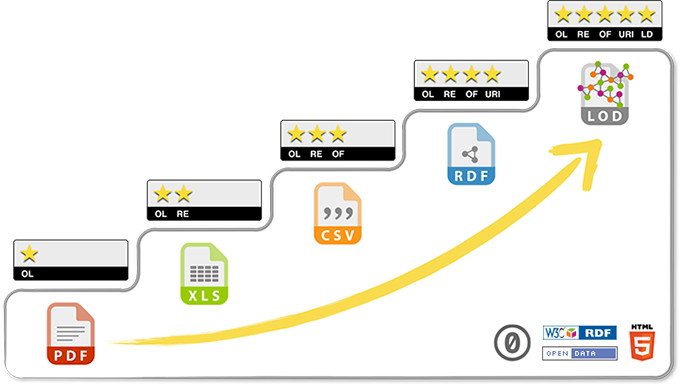
\includegraphics[scale=0.5]{images/5-star-steps.png}
    \centering
	\caption[The 5 star steps of Linked Data]{The 5 star steps of Linked Data.}
	\label{fig:margin-5-star-steps}
\end{figure}

Similar to this four principles is the 5 stars Linked Open Data Model, illustrated in \cref{fig:margin-5-star-steps}.
RDF is mentioned in the third principle as one of the standards that provides useful information. The goal of this
principles is that data is not only ready for humans to navigate through but also for other agents, like computers,
that may automatically process that data.

All the above motivations helped to make RDF the language for the Web of Data, as described in \cite{labra-validating-rdf}.
And the main features that it presents are: \textit{Disambiguation}, \textit{Integration}, \textit{Extensibility}, \textit{Flexibility} and \textit{Open by Default}.
With the features also some drawbacks are associated, the most important one and the one we will focus is the RDF
\textbf{production/consumption dilemma}.

RDF production/consumption dilemma states that it is necessary to find ways that data producers can generate their data so
it can be handled by potential consumers. For example, they may want to declare that some nodes have some properties with
some specific values. Data consumers need to know that structure to develop applications to consume the data.

Although RDF is a very flexible schema-less language, enterprise and industrial applications may require an extra level of
validation before processing for several reasons like security, performance, etc.

To solve that dilemma and as an alternative to expecting the data to have some structure without validation, Shape Expressions Language
\textit{(ShEx)} was proposed as a human-readable and high-level open source language for RDF validation. Initially, ShEx was proposed
as a human-readable syntax for OSLC Resource Shapes \cite{oslc-resource-shape} but ShEx grew very fast to embrace more
complex user requirements coming from clinical and library use cases.

Another technology, SPARQL Inferencing Notation (SPIN) \cite{knublauch2011spin}, was used for RDF validation, principally in TopQuadrant’s TopBraid Composer. This technology, influenced
from OSLC Resource Shapes as well, evolved into both a private implementation and open source definition of the SHACL
\textit{(Shapes Constraint Language)}, which was adopted by the W3C Data Shapes Working Group.

From a user point of view the possibilities of ShEx are very large, from the smallest case to just validate a node with one property
to a scientific domain case where we need to validate the human genome\footnote{\url{https://github.com/geneontology/go-shapes}}. A language with such a number
of possibilities requires from a strong syntactic and semantic validation and that leads us to our first goal.

\begin{researchquestion}
  Determine how much the existing syntactic and semantic validation systems for shape expressions can be enhanced. And
  if existing systems can be enhanced propose a prototype that implement those enhancements.
\end{researchquestion}

Secondly and very related to programming languages, if we take the PopularitY of Programming Language \textit{(PYPL)} Index\footnote{\url{http://pypl.github.io/PYPL.html}}
from June 2020 we can see that more than half of the share is occupied by languages that support the object oriented paradigm. And therefore this paradigm
becomes the most used one. The aim of this paradigm is to model real world domains, according to \cite{wegner1990concepts}. That, in fact, is the same goal
that ShEx has, it allows to model real world domains with schemas, and validate existing data with them. Therefore our second goal relies on this and tries
to automatically transform shape expressions into object domain models coded in any language that supports the object oriented paradigm:

\begin{researchquestion}
  Determine till which point can we automatically translate existing shape expressions to object domain models. And
  propose a prototype capable of translating Shape Expressions to object domain models.
\end{researchquestion}

If this were possible it would not only imply that you could automate the creation of application domain models but that you could link the domain model that an
application uses with a domain model defined through Shape Expressions that describes the schema of a RDF data set.

\bigskip

To give answers to the questions posed in this section, we will limit our scope to the micro grammar of Shape Expressions, defined in
\footnote{\url{https://dcmi.github.io/dcap/shex_lite/micro-spec.html}}. This version is a strict subset of the complete ShEx grammar
and therefore any derived method or technology we can draw from it can automatically be applied to the full grammar.

% S E C T I O N   C O N T R I B U T I O N S

\section{Contributions}
\label{sec:intro-contri}
These are the major contributions of this dissertation:

\begin{enumerate}
  \item A parser for the ShEx micro Compact Syntax. There are already existing parsers for ShEx and they work for ShEx micro Compact Syntax
  as it is a subset of ShEx, but they accept more structures than the ones defined by ShEx micro Compact Syntax. We propose a parser that
  is only focused on ShEx micro Compact Syntax and therefore error and warning messages can be enhanced.
  
  \item Error and warning analyser for schemas. Existing approaches do not semantically validate the schemas, they
  only perform error detection by means of complex grammars and parsers. Our proposed system does semantically validate the schemas by means
  of a custom analyser that performs both syntactic and semantic analysis so it produces human-friendly errors and warnings that users can
  use to fix their schemas.

  \item Automatic translation of schemas into object domain models in \texttt{Java} and \texttt{Python}. The proposed system
  integrates an open back-end with built-in code translation from the validated schemas to domain models in Object
  Oriented Programming Languages \textit{(OOPL)} \cite{oopl}.

  \item Evaluation of errors and warnings generated of our proposed solution against existing tools. This comparison
  empirically shows the benefits and drawbacks of our proposed system.
\end{enumerate}

% S E C T I O N   S T R U C T U R E   O F   T H E   D O C U M E N T

\section{Structure of the Document}
\label{sec:intro-structure}
The dissertation layout is as follows:
\bigskip

\begin{description}
  \item[\cref{ch:theo-back}] Indicates the state of the art of the existing RDF validation technologies, tools for processing Shape
  Expressions and other related projects.
	\item[\cref{ch:retalted-work}] Gives a basic theoretical background that it is needed to fully understand the concepts explained in the
  following chapters.
  \item[\cref{ch:current-analysers-analysis}] Analyses current syntactic and semantic analysis systems.
  \item[\cref{ch:proposed-sin-sema-anal}] He proposes a system by means of software engineering techniques
  that tries to solve the problem posed in the previous chapter.
  \item[\cref{ch:proposed-implementation}] It proposes an implementation that meets the expectations of the previous chapter.
  This implementation is the one that will be used to carry out the evaluation of results.
  \item[\cref{ch:odm-transl}] Define the ShEx translation problem to object-oriented languages and compare the
  expressivities of both systems.
  \item[\cref{ch:proposed-translator}] It focuses on proposing a solution to the problem raised in the previous chapter.
  First through formalizations and then employing software engineering methodologies.
  \item[\cref{ch:proposed-system}] It offers a proposed implementation to meet the expectations of the previous chapters.
  This implementation will be used to evaluate the results.
  \item[\cref{ch:results-evaluation}] It defines a methodology and the data on which the methodology will be tested. Then evaluate the results obtained.
  \item[\cref{ch:planning-and-budget}] It includes the description of the project planning as well as its cost budget.
  \item[\cref{ch:conclusions}] It summarizes the results achieved after completing the work and includes the proposals for future work.
\end{description}